\documentclass[tikz,border=10pt]{standalone}
\usepackage{tikz}
\usetikzlibrary{shapes,positioning}

\begin{document}
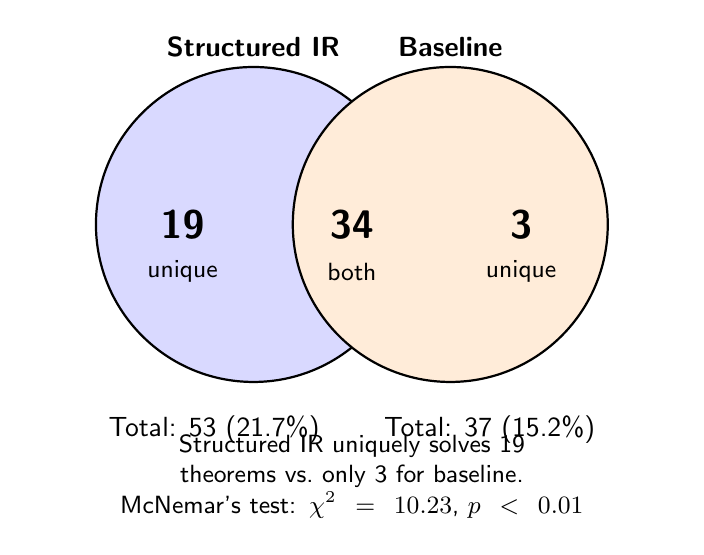
\begin{tikzpicture}[
    every node/.style={font=\sffamily},
    set/.style={circle, minimum size=4cm, draw, thick}
]

% Draw the two circles
\node[set, fill=blue!15, label={[font=\sffamily\bfseries]above:Structured IR}] (A) at (0,0) {};
\node[set, fill=orange!15, label={[font=\sffamily\bfseries]above:Baseline}] (B) at (2.5,0) {};

% Labels with counts
\node[font=\sffamily\Large\bfseries] at (-0.9,0) {19};
\node[font=\sffamily\small, text width=1.2cm, align=center] at (-0.9,-0.6) {unique};

\node[font=\sffamily\Large\bfseries] at (1.25,0) {34};
\node[font=\sffamily\small] at (1.25,-0.6) {both};

\node[font=\sffamily\Large\bfseries] at (3.4,0) {3};
\node[font=\sffamily\small, text width=1.2cm, align=center] at (3.4,-0.6) {unique};

% Totals below
\node[font=\sffamily, anchor=north] at (-0.5,-2.3) {Total: 53 (21.7\%)};
\node[font=\sffamily, anchor=north] at (3.0,-2.3) {Total: 37 (15.2\%)};

% Caption
\node[font=\sffamily\small, text width=8cm, align=center] at (1.25,-3.2) {
    Structured IR uniquely solves 19 theorems vs.\ only 3 for baseline.\\
    McNemar's test: $\chi^2 = 10.23$, $p < 0.01$
};

\end{tikzpicture}
\end{document}
